\section{Hosts with their own dynamics}\label{sec:dyn}

\paragraph{In brief.}
Once an established parasite changes host abundance, stability concerns whether small disturbances decay around an endemic equilibrium. The response of each host and parasite stage determines this local stability. When a parasite depresses a self-regulated host below the density of peak production, intermediate external-stage durations can destabilize an equilibrium that is stable at shorter and longer durations.

Once a parasite establishes in hosts that it harms, stability concerns the decay of disturbances around a positive endemic equilibrium \citep{anderson1978,dobson2020}. We analyze continuous-time hosts with births, deaths, and density dependence. The models are deterministic except in Section~\ref{subsec:dyn-noise}. An equilibrium is \emph{stable} when its Jacobian is Hurwitz (every eigenvalue has negative real part). A positive real part gives linear instability; zero or purely imaginary eigenvalues decide neither nonlinear outcome. Derivatives and gains are evaluated at equilibrium, rates have units of inverse time, and responses are dimensionless. Local symbols ($A, B, C, J, U, V_0, q, d, h, \mathcal{T}$) differ from those in Sections~\ref{sec:ring}--\ref{sec:exact}.

\subsection{Response blocks, the characteristic polynomial, and damping}\label{subsec:dyn-blocks}

A ring of $n\ge1$ blocks passes scalar infection pressure $u_k$ into block $k$ and output $v_k=u_{k+1}$ to the next block, without direct host interactions. Relative perturbations $x_k=\delta u_k/u_k^*$ and $y_k=\delta v_k/v_k^*$ satisfy $y_k(z)=E_k(z)x_k(z)$ at complex rate $z$. We retain the full internal characteristic polynomial in $E_k(z)=N_k(z)/D_k(z)$ and leave the numerator unreduced. The five blocks were derived twice and proved in Appendix~\ref{app:dyn} (Table~\ref{tab:dyn-blocks}; validation details in Online Resource 1). Block V requires $a\ge\alpha$, because parasite-killed hosts leave both $N$ and $I$.

\begin{table}[ht]
\caption{Continuous-time response blocks at a positive equilibrium ($a, c, \xi, \lambda_P > 0$, $\alpha \ge 0$)}\label{tab:dyn-blocks}
\footnotesize
\begin{tabular*}{\textwidth}{@{\extracolsep\fill}lp{0.32\textwidth}p{0.26\textwidth}p{0.25\textwidth}@{}}
\toprule
Block & \raggedright Nonlinear equations and output & \raggedright Response $E(z) = N(z)/D(z)$ & \raggedright Qualification (Prop.~\ref{prop:dyn-k3}) \tabularnewline
\midrule
L & \raggedright $\dot{w} = u - aw,\; v = cw$ & \raggedright $a/(z + a)$ & \raggedright $|E(\mathrm{i}\omega)| \le 1$; non-amplifying \tabularnewline
R$^{\mathrm{a}}$ & \raggedright $\dot{w} = u - aw,\; v = cf(w)w$ & \raggedright $(1 - \kappa)a/(z + a)$ & \raggedright Non-amp.\ $0 \le \kappa \le 2$; damping $0 < \kappa < 2$ \tabularnewline
S$^{\mathrm{b}}$ & \raggedright $\dot{I} = u(N - I) - aI,\; v = cI$ & \raggedright $a/(z + d),\; d = a/(1 - p)$ & \raggedright $|E(\mathrm{i}\omega)| \le 1 - p$; damping \tabularnewline
V$^{\mathrm{b}}$ & \raggedright $\dot{N} = \Phi(N) - \alpha I,\; v = cI,$ $\dot{I} = u(N - I) - aI$ ($a \ge \alpha$) & \raggedright $q(z + \rho)/D(z)$ ($q = a$, $d = a/(1-p)$, $h = \alpha p$) & \raggedright For $\rho \ge 0$: $|E(\mathrm{i}\omega)| \le 1 - p$; damping if $\rho + h > 0$ \tabularnewline
M$^{\mathrm{c}}$ & \raggedright $\dot{H} = \Phi(H) - \alpha P,\; v = \lambda_P P,$ $\dot{P} = uH - \xi P - \alpha\varepsilon P^2/H$ & \raggedright $q(z + \rho)/D(z)$ ($h = \alpha m$, $q = \xi + \varepsilon h$, $d = \xi + 2\varepsilon h$) & \raggedright For $\rho \ge 0$: $|E(\mathrm{i}\omega)| \le q/d$; damping if $h > 0$ \tabularnewline
\bottomrule
\end{tabular*}
\par\smallskip\noindent\footnotesize
$^{\mathrm{a}}$Evaluated with $f(w^*) > 0$ and elasticity $\kappa = -w^* f'(w^*)/f(w^*)$; $D(z) = z + a$ for L and R.
$^{\mathrm{b}}$Prevalence $p = I^*/N^* \in (0, 1)$; for V and M, $D(z) = (z + \rho)(z + d) + dh$ with $\rho = -\Phi'(X^*)$ at $X^* = N^*$ or $H^*$.
$^{\mathrm{c}}$After \citet{anderson1978}; mean burden $m = P^*/H^* > 0$, aggregation $\varepsilon \ge 1$. Exact V and M tests are in~\eqref{eq:dyn-uv}.
\end{table}

For dynamic hosts ($X = N$ or $H$), let $\rho = -\Phi'(X^*)$ and define
\begin{equation}\label{eq:dyn-abjc}
A = \rho + d, \qquad B = d(\rho + h), \qquad J = \rho + d - q, \qquad C = \rho(d - q) + dh.
\end{equation}
Equilibrium of $\dot{X}$ and differentiation of per-capita net production give
\begin{equation}\label{eq:dyn-slope}
h = \frac{\Phi(X^*)}{X^*}, \qquad \rho + h = -X^* \left.\frac{\dd}{\dd X}\frac{\Phi(X)}{X}\right|_{X = X^*}.
\end{equation}
Thus $\rho \ge 0$ means the host is held on the falling side of total net production, whereas $\rho + h > 0$ means per-capita self-regulation. Under logistic growth $\Phi(X) = rX(1 - X/K)$, a host depressed below $K/2$ has $-h < \rho < 0$, $\rho + h > 0$, and negative static response $E(0) < 0$ (over-compensation). At $\rho = -h$, per-capita production has zero local slope, with $\Phi(X) = rX$ as one example. Admissibility ($a \ge \alpha$ for V, $\varepsilon \ge 1$ for M) gives $d - q \ge h$, hence $A, J > 0$ for $\rho > -h$ and, at $\rho=-h$, $J>0$ for V, while for M, $J=(\varepsilon-1)h$ is positive exactly when $\varepsilon>1$ and $h>0$.

The full characteristic polynomial retains all disturbance modes, including those that a simplified response equation can omit (Proposition~\ref{prop:dyn-k1}, Appendix~\ref{app:dyn}).

Proposition~\ref{prop:dyn-k1} was proved in Appendix~\ref{app:dyn} and refereed. Cross-block cancellation, unobservable modes, or a zero numerator can omit roots from $\prod_kE_k(z)=1$, so the full polynomial is needed. A worked example and numerical checks are in Online Resource 1.

A block is \emph{non-amplifying} if its internal matrix is Hurwitz and $|E(\mathrm{i}\omega)| \le 1$ for all $\omega \in \mathbb{R}$, and \emph{damping} if the inequality is strict for all $\omega \in \mathbb{R}$.

\begin{theorem}[Stability of non-amplifying rings]\label{thm:dyn-k2}
If every block in a scalar-coupled ring is non-amplifying at the equilibrium and at least one block is damping, the ring is Hurwitz for any $n \ge 1$ and any positive time constants.
\end{theorem}

Theorem~\ref{thm:dyn-k2} was proved in Appendix~\ref{app:dyn} and refereed. Both hypotheses are needed: an all-L ring has a zero eigenvalue, and amplifying blocks can destabilize a ring containing a damper (example and checks in Online Resource 1).

The response criteria identify which host and parasite stages damp disturbances and which can amplify them (Proposition~\ref{prop:dyn-k3}, Appendix~\ref{app:dyn}).

Proposition~\ref{prop:dyn-k3} was proved in Appendix~\ref{app:dyn} and refereed (checks in Online Resource 1). Its qualifying rings are stable for any host count or durations. Nonnegative $\rho$ is sufficient, not necessary. For logistic production it requires $X^*\ge K/2$, which small parasite-induced mortality alone does not establish. Applications therefore require the host production curve and endemic density.

\subsection{Host depression, stage duration, and constant-number hosts}\label{subsec:dyn-delays}

Depressing a self-regulated host below peak total production ($-h < \rho < 0$) can open a bounded unstable range of external stage durations (proved in Appendix~\ref{app:dyn} and refereed).

\begin{proposition}[Self-regulated host and one delay]\label{prop:dyn-k4}
For one V block ($a_V \ge \alpha$) or M block ($\varepsilon \ge 1$) and one L block of rate $a_L > 0$ with $c_L/a_L$ and the equilibrium fixed, $\chi(z) = z^3 + (a_L + A)z^2 + (B + a_L J)z + a_L C$. When $-h < \rho < 0$, we have $A, B, C, J > 0$ and stability holds if and only if
\begin{equation}\label{eq:dyn-fquad}
F(a_L) = (a_L + A)(B + a_L J) - a_L C = J a_L^2 + (AJ + q\rho)a_L + AB > 0.
\end{equation}
Small and large $a_L$ are stable, and an open interval $a_- < a_L < a_+$ is unstable if and only if $q|\rho| - AJ > 2\sqrt{JAB}$, with
\begin{equation}\label{eq:dyn-island}
a_\pm = \frac{q|\rho| - AJ \pm \sqrt{(q|\rho| - AJ)^2 - 4JAB}}{2J},
\end{equation}
a single nonhyperbolic rate at equality, and boundary frequency $\omega^2 = B + a_L J = a_L C/(a_L + A)$.
\end{proposition}

An illustrative V host has instability for $0.0456087<a_L<1.9326281$, confirmed by stiff nonlinear integrations on both sides (Fig.~\ref{fig:dyn-1}; parameters and numerical checks in Online Resource 1).

\begin{figure}[ht]
\centering
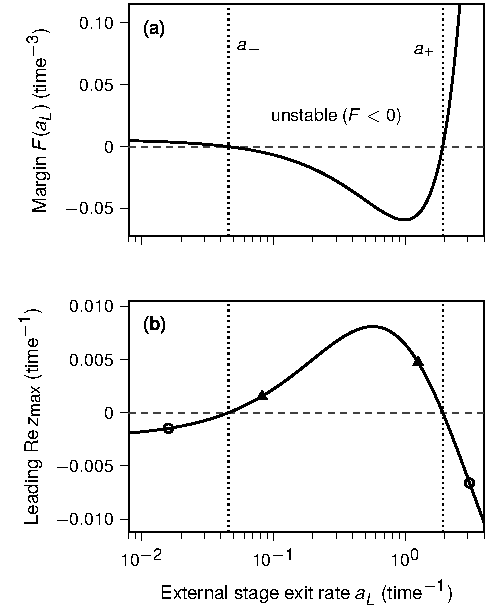
\includegraphics[width=84mm]{figures/dyn-1.pdf}
\caption{Island of instability for an illustrative depressed host ($a_V = 1.05$, $\alpha = 1$, $p = 0.20$, $h = 0.20$, $\rho = -0.196$) and one external L stage of rate $a_L$ with $c_L/a_L$ fixed. (a) Routh--Hurwitz margin $F(a_L)$ from~\eqref{eq:dyn-fquad} (solid curve), zero line (dashed), and roots $a_- = 0.0456087$, $a_+ = 1.9326281$ (dotted). (b) Leading eigenvalue real part $\operatorname{Re} z_{\max}$ (solid curve) and stiff nonlinear perturbation rates (circles for decay at $a_L = 0.0160, 3.0922$; triangles for growth at $a_L = 0.0821, 1.2562$)}\label{fig:dyn-1}
\end{figure}

For one V or M host without first-order self-regulation ($\rho=-h$, $h>0$), lengthening one external stage at fixed equilibrium and static gain cannot restore lost local stability (Proposition~\ref{prop:dyn-k5}, Appendix~\ref{app:dyn}). When the rest of the ring consists only of L stages, a chain of two stages with equal, sufficiently small exit rates is unstable for $A>0$, and every nonempty finite chain is unstable when $J\leq0$. These conclusions are restricted to rings whose remaining blocks are all L; adding damping blocks such as S can change the stability test. For one host and one L stage with fixed $d,q,h$, $d>h$, and $qd>(d-h)^2$, the lower critical rate is proportional to weak self-regulation $\delta=\rho+h$ as $\delta\downarrow0$ (the same proposition; checks in Online Resource 1).

More generally, when every other block is internally stable and its response is held fixed, write $Q(0)$ for the product of their zero-frequency responses. At fixed equilibrium and static gain, one sufficiently slow external stage stabilizes the ring if $Q(0)<1$. If $Q(0)>1$, the ring has a positive real eigenvalue at every external-stage rate; if $Q(0)=1$, it has a zero eigenvalue (Proposition~\ref{prop:dyn-k6}, Appendix~\ref{app:dyn}; refereed, checks in Online Resource 1).

One slow stage thus stabilizes even strong single-host over-compensation when the host block is internally stable ($Q(0)<0$). The appendix gives two contrasting examples: two internally stable over-compensating V blocks with $Q(0)=4$ remain unstable with one L stage, and one such V block is unstable with eight equally slow L stages. In over-compensating regulated (R/L) rings with negative total feedback and $n\geq3$, stage exit rates that are not all equal raise the critical feedback strength above its equal-rate value $\sec^n(\pi/n)$ (Proposition~\ref{prop:dyn-k7}, Appendix~\ref{app:dyn}). This criterion is published cyclic-feedback theory \citep{sontag2006,arcak2006,arcak2008,nguyen2009,hori2011,ananthasubramaniam2014} (proved in Appendix~\ref{app:dyn} and refereed; not found for parasite cycles in our search).

Constant-number hosts damp the loop, but comparisons of return speed depend on which total duration is held fixed (Proposition~\ref{prop:dyn-k8}, Appendix~\ref{app:dyn}).

\subsection{Noise response, boundary counts, and formal checks}\label{subsec:dyn-noise}

Near a Hurwitz equilibrium, transfer functions describe weak stationary infection-pressure forcing \citep[compare][]{roberts1992,marion2000}. The result was derived twice, refereed, and proved in Appendix~\ref{app:dyn}; simulation checks are in Online Resource 1.

For constant-number hosts linked by external stages, lengthening one stage at fixed equilibrium, gains, and other rates can filter weak stationary forcing along paths through it. This filtering does not remove forcing that is slow relative to both the stage and the rest of the ring's response (Proposition~\ref{prop:dyn-k9}, Appendix~\ref{app:dyn}).

This is a first-order response; no nonlinear remainder is supplied.

First Lyapunov coefficients were negative at all 900 sampled V boundaries, while M boundaries had both signs (computed once). Crossing speed and remaining eigenvalues were not checked across the sample, so these counts do not certify Hopf bifurcations. Details and nonlinear checks are in Online Resource 1.

Under their stated model and textbook assumptions, Lean~4 checks the complete statements of Proposition~\ref{prop:dyn-k1}, Theorem~\ref{thm:dyn-k2}, and Proposition~\ref{prop:dyn-k8}. For Propositions~\ref{prop:dyn-k3}, \ref{prop:dyn-k4}, and~\ref{prop:dyn-k5}, it checks every conclusion that follows from the linearized block responses, which enter the Lean files as stated rather than being derived there from the nonlinear block equations. It checks specified components of Propositions~\ref{prop:dyn-k6}, \ref{prop:dyn-k7}, and~\ref{prop:dyn-k9}. The checked declarations use no \texttt{sorry} or nonstandard axioms. Table~\ref{tab:dyn-lean} summarizes the stability results. The scope and remaining gaps are recorded in the reconciled coverage inventory archived with the Lean sources (see Code availability).

\subsection{Published grouse--nematode models and Dobson's trophic model}\label{subsec:dyn-models}

The model of \emph{Trichostrongylus tenuis} in red grouse (\emph{Lagopus lagopus scoticus}) of \citet{dobson1992} (read in full; field background \citealp{hudson1992}) and two regimes after \citet{gaba2008} fall outside the two-state V/M plus external L blocks \citep[compare][]{may1978,rosa2002}. Territorial regulation and fecundity loss affect the host response, and arrested larvae require a three-state host block. Changing durations also alters survival, $R_0$, and equilibrium host density. Additionally, host uptake directly depletes free-living larvae. Pairing the three-state response with a scalar L block reproduced the tested territorial transitions, but missed restabilization at long arrestment without territorial regulation or fecundity loss. Omitting larval-uptake saturation caused this discrepancy. These comparisons were computed once; worked examples and validation are in Online Resource 1 (Table~\ref{tab:dyn-grouse}).

Direct coupling between predator and prey hosts also breaks the scalar ring \citep{dobson1988,hadeler1989,fenton2006,rogawa2018}. Run R11 analyzed one pre-registered, dimensionally consistent reading of equations 1.6--1.11 of \citet{dobson2020} (computed once; protocol and tallies in Online Resource 1).

\begin{figure}[ht]
\centering
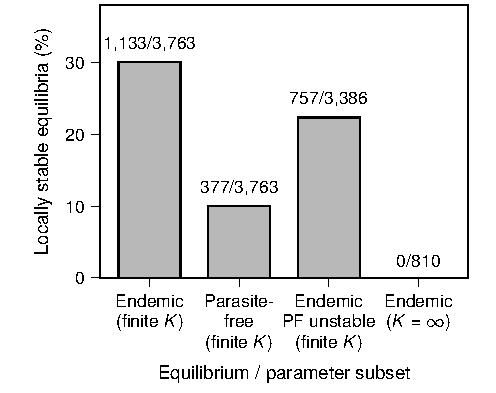
\includegraphics[width=84mm]{figures/dyn-2.pdf}
\caption{Local stability shares for the endemic system and parasite-free host subsystem in trophic sweep R11 with corrected finite-$K$ and $K = \infty$ denominators, showing endemic ($1{,}133/3{,}763 = 30.1\%$) and parasite-free host-subsystem ($377/3{,}763 = 10.0\%$) shares across finite-$K$ sets, endemic stability among host-subsystem-unstable finite-$K$ sets ($757/3{,}386 = 22.4\%$), and endemic stability for $K = \infty$ ($0/810 = 0.0\%$)}\label{fig:dyn-2}
\end{figure}

For self-limited prey, the endemic equilibrium was stable in $30.1\%$ of cases, compared with $10.0\%$ for the parasite-free subsystem (Fig.~\ref{fig:dyn-2}). None of 810 baseline endemic equilibria without prey self-limitation was stable. Longer free-living durations generally reduced stability in the tested comparisons. Stability was associated with greater relative prey density, but no threshold was established. Matched direct cycles were more often stable than trophic cycles. These are numerical findings from this sample; comparisons, uncertainty estimates, and restrictions are in Online Resource 1.

These results indicate that endemic stability depends on host production at the infected density, the location of delays, and direct predator--prey interactions. Host count and $n$th roots of $R_0$ do not determine these quantities.
